This chapter consists of two parts. The first part will provide an evaluation of the Matrix security model and relies on the paper \emph{SoK: Secure Messaging} \cite{sok} and \emph{The Olm Cryptographic Review} by NCC Group \cite{ncc}. 

The second part provides a preliminary analysis of the IFC tools, the selection of Paragon and the rationale behind it, and a further analysis of the selected tool Paragon.


\section{Evaluation of Matrix security model}
The security of matrix will be evaluated in the context of secure messaging. An evaluation framework has been proposed in the paper \emph{SoK: Secure messaging} which the evaluation will be loosely based on. 

The evaluation framework covers several areas with \emph{conversation security} being the most relevant for this evaluation. The area \emph{conversation security} describes three categories; \emph{Security and Privacy}, \emph{Adoption}, and \emph{Group Chat}. Obviously the most relevant category for the evaluation is \emph{Security and Privacy}

\subsection{Threat model}
For secure messaging the evaluation framework defines a threat model with three types of adversaries:

\begin{itemize}
	\item \emph{Local adversary:} The adversary is in control of the local network.
	\item \emph{Global adversary:} The adversary is in control of great portions of the Internet 
	\item \emph{Service providers:} A potential adversary for messaging systems with centralized infrastructure.
\end{itemize}
Note that an adversary can be of several types.
In the messaging system the adversary may be a participant with the following properties:

\begin{itemize}
	\item An adversary can start a conversation.
	\item An adversary can send messages.
	\item An adversary can perform any other action that a participant is capable of.
\end{itemize}

Finally we assume that the endpoints in a secure messaging system are secure.

This evaluation will inherit the described threat model.

\subsection{The Signal Protocol}
Matrix provides end-to-end encryption by using the Olm and Megolm library with the former being an implementation of the Double Ratchet algorithm also known as the Signal Protocol, and the latter being the algorithm used for group chat. 

Olm is used for securely exchanging message keys/session keys during group chat and is vital part of the end-to-end encryption in Matrix.

Before the Matrix protocol is evaluated the Signal Protocol will be considered. 

Section xx provides a list of security properties relevant for \emph{conversation security}. These security properties is used for evaluating a secure messaging protocol such as the Signal Protocol.
%Any messaging application that provides end-to-end encryption is likely an implementation of  the protocol 

The table below shows an evaluation of the Signal Protocol (previously known as TextSecure) \cite{sok}. 

\begin{figure}[H]
	\hspace*{-1.7cm} 
	\centering
	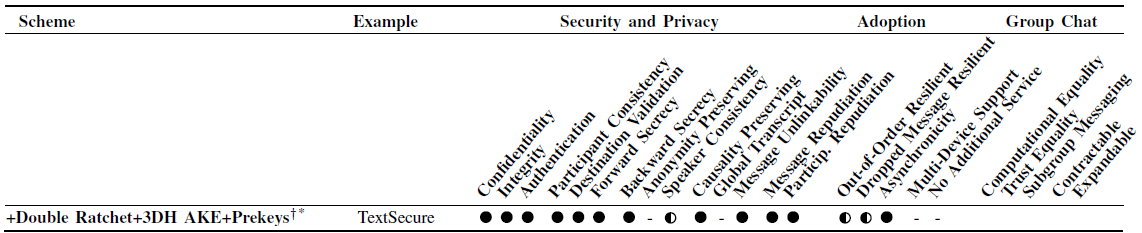
\includegraphics[width=16cm]{figures/framework_signal.png}
	\caption{Evaluation of Signal (TextSecure) \cite{sok}.}
	\label{fig:framework_signal}
\end{figure}


%Explain how they provide the properties or why they don't


\subparagraph{Confidentiality} When a message is sent using the Signal Protocol then only the intended recipient can read the message. The senders sending ratchet and receivers receiving ratchet will derive the same message key hence only the two parties will be able to encrypt the messages. 

\subparagraph{Integrity} The receiver will only accept a message if it is successfully decrypted hence if in transit a message was modified then the message would be rejected.

\subparagraph{Authentication} The decryption of a message also gives authentication guarantees since only the intended recipient could compute the message key.

\subparagraph{Forward secrecy} The symmetric ratchet ensures forward secrecy. If a chain session key is compromised then the previous keys can not be generated since the ratchet is one way cryptographic hash function hence secrecy is provided for all previous send messages.  

\subparagraph{Backward secrecy} Diffie-Hellman ratchet have the self-healing property and will generate a new chain session key for the symmetric ratchet hence if a chain key is compromised then secrecy for future messages is still provided because a new chain ratchet key will be generated.

\subparagraph{Anonymity preserving}

Anonymity preservation is lost in the Signal Protocol since the initial key agreement requires long-term public keys hence making them observable during Triple-DH. However \textbf{\emph{participant consistency}} is provided by Triple-DH \cite{sok}. %How?
%Without participant consistency, identity misbinding attacks might be possible. Unknown key share attack

\subparagraph{Speaker consistency}
This property is partially provided through the key evolution of the ratchets. If a message is dropped then it is not possible to generate message keys for future messages. This also makes the protocol partially have the property \emph{\textbf{Dropped message resilence}}. It will also not go unnoticed if a message is received out of order since this will result in the message's key being an unexpected key. Hence the recipient have to store expired keys to decrypt delayed messages. This makes the property \emph{\textbf{Out-of-order resilient}} only partially provided \cite{sok}.

\subparagraph{Global transcript} 
In an asynchrounous messaging protocol there is no global transcript. Both participants have to be online to receive messages hence the participants will not have all the messages if one of them is offline. This is a result of having the \textbf{\emph{Asynchronicity}} property.

\subparagraph{Deniability properties}

Since the ratchet session keys are used for encrypting messages and not the long-term public keys the properties \textbf{\emph{Message unlinkability}} and \textbf{\emph{Message repudiation}} are provided. 


\subparagraph{Other properties}

\begin{itemize}
	\item \textbf{\emph{Participant repudiation}}. Triple-DH achieves full participant repudiation since anyone can forge a transcript between any two participants \cite{sok}.
	\item \textbf{\emph{Destination validation}}. The Deffie-Hellman ratchet provides this property since the recipients public key is used to generate the chain key \cite{sok}. % Is this true?
\end{itemize}


The evaluation shows that several security properties are provided with the important ones being confidentiality, integrity, authentication, forward secrecy, backward secrecy. 

Furthermore a formal analysis have been made on the Signal Protocol that proves the protocol is free from any major flaws and it satisfy the following security properties; confidentiality, authentication and secrecy \cite{Signal}. 

\paragraph{Application variants}

The Signal Protocol is a secure messaging protocol and have been extensively studied including proof that the standard security properties are assured. 

The Olm library used by Matrix is a variant of the Signal Protocol. There is no implementation analysis of the Olm library hence there is no guarantee that all the security properties defined in xx is inherited by Olm.

The further evaluation relies upon the the security assessment of Matrix. 


%The next section provides a brief summary of the analysis.

%\newpage
%
%\subsubsection{Summary of the security analysis of Signal Protocol}
%\emph{**NOTE: Is this section even relevant to have in the report? **}
%
%
%As described earlier in section xx the Signal Protocol consists of three stages.
%
%\begin{itemize}
%	\item Initial stage (Triple-DH). For establishing a shared secret. 
%	\item Deffie-Hellman ratchet. For generating session key. 
%	\item Symmetric ratchet. For generating message key.
%\end{itemize}
%
%
%
%\paragraph{Threat model}
%The threat model defined in the analysis assumes that the adversary have full control over the network.
%
%The adversary can observe traffic over the network and can drop and send messages.
%
%For an adversary to break security he must be able to
%
%For an adversary to break security he must obtain 
%
%In assymmetric messaging a party can be offline over 
%
%\paragraph{Security properties}
%
%The high-level properties we aim to prove are secrecy and authentication of message keys
%
%\begin{itemize}
%	
%	\item Secrecy. If Alice and Bob complete an exchange to generate a key k, nobody other than Alice and Bob should be able to learn anything about k. Forward secrecy are not explicit goals; instead, derived session keys should remain secret under a variety of compromise scenarios.
%	\item (Implicit) Authentication. If Alice believes that she shares the key k with Bob, nobody other than Bob should be able to learn anything about k. Note that this property is implied by secrecy. Authentication will be implicit meaning that only the intended party could compute the key rather than explicit (get a guarantee that the intended party did compute the key).
%\end{itemize}
%
%%and thereby distinguish any fresh message encryption key from random
%
%
%As described earlier a group chat is represented by a session which has three stages; initial exchange, asymmetric and symmetric. Each stage will generate a key 
%
%
%By proving that the session keys generated at each stage are key indistinguishable it can be argued that the session keys at each stage are safe...
%
%
%We find if the above goals are fulfilled by looking at the freshness of the session keys in the different stages. By defining under what conditions the session keys are fresh and by proving that they indeed are fresh then it has been proved that the above security properties are provided. 
%
%
%\paragraph{Freshness and cleanness} 
%
%Our goal when defining fresh is to describe the best security condition that might be provable for each of
%Signal’s message keys based on the protocol’s design; here, “best” is with respect to the maximal combinations
%of secrets learned by the adversary.
%That is, we use the structure of the protocol to infer which attacks cannot
%possibly be prevented, and rule them out by restricting the adversary.
%
%For each session there are different definition of freshness.
%
%The cleanness predicate defines under what conditions the session keys are .....
%
%
%
%\subparagraph{Stage 0}
%We can prove the security of the stage 0 key (output by the triple key exchange during session setup) if one of the following is upheld cleanLM(u,i), cleanEL(u,i,0), cleanEM(u,i,0).
%
%\subparagraph{Asymmetric stages}
%In this stage there are two types; asym-ir (sending) or asym-ri (receiving).
%
%By satisfying the cleanness predicates for each type of state we can prove the security of this stage.
%
%Most cases are of the form cleanEE, and for these we obtain a probability bound by replacing the DH ratchet keys and shared secrets with values from a GDH challenger.
%
%The only case not of this form involves clean\_state, which describes a scenario where both recent ratchet keys were compromised but the previous stage was still secure. Secrecy here is intuitive, and the bound follows from an inductive argument: if an adversary could win in this manner, then, assuming GDH and ROM security, there is an adversary which could win against the previous stage.
%
%
%\subparagraph{Symmetric stages}
%To ensure security of session key in this stage we only need to consider the following case. We replace the keys used to initialise the current sending chain with uniformly random values, since an adversary who could detect this could win against that
%previous stage.
%\\
%\\
%The proof for the above is provided in detail in the paper \emph{A Formal Security Analysis of the Signal Messaging Protocol} \cite{Signal}.



\subsection{Matrix protocol}

(Olm) is great at encrypting conversations between pairs of devices, but it starts to get a bit unwieldy when you use it for a group conversation – especially the huge ones we have in Matrix.  Either each sender needs to encrypt each message N times for every device in the room (which doesn’t scale), or you need some other mechanism.

How megolm works..




List problems with group chat 

\begin{itemize}
	\item Lack of post compromise security
\end{itemize}

There is an tradeoff on security and usability and the security is decreased for group chats. %8.30

As of this moment of writing there exist no implemented protocol that solves these issues in group chat. However recent research has proposed solutions with early implementations for these problems with IETF leading the research on the standard on \emph{Messaging Layer Security}. Matrix has expressed awareness of the protocol and a possibility of adaption in the future.

\subsubsection{Olm}
Olm is an implementation of the Double Ratchet algorithm and plays a major role in the Megolm library which is used by Matrix group messaging. 

The security assessment provides a review of the Olm and Megolm libraries. However there exist no work that verifies if Olm correctly implements the Double Ratchet described earlier.

Vulnerabilities found in the security assessment. 

\paragraph{Unknown Key Share attack}

In this variant of the unknown key-share (OKs) attack, an attacker will allow highly targeted, known messages to be sent to Bob. In this scenario, Bob will still believe he is talking with Alice. Here, two parties (Donald and Mallory), who may be the same person, will collude against Alice in a group chat situation (Megolm). Donald will be performing the unknown key-share attack. Mallory will be an instigator (attempting to elicit messages from Alice that will later be sent to Bob) who will be able to read the contents of the group chat.

\subsubsection{Megolm}

Each sender has a sender ratchet (Megolm Ratchet). Each recipient has a corresponding receiving ratchet for each sender. So if there are three participants in a group then each participant will have two receiving ratchet. When a session is started a sender will send his initial ratchet key to each recipient, so that the sender ratchet and each recipients ratchet are in sync. This key exchange happens over a secure communication channel (Olm). Also this generates a burst of sending N initial messages when a session is initiated (where N is the number of participants). Until a new session is started no further session keys are exchanged and the corresponding message keys are generated by incrementing the ratchet.

When a sender sends a message a message key is generated from the ratchet key and the message is encrypted using that message key. The message will be signed so the recipient will know which sender the message is from and which ratchet to utilize. %(not with a long-term I guess? hence providing deniability)
The message  is then send to the server which relays the message to all recipients over an insecure channel. When they receive the message the same message key is generated using the corresponding receiver ratchet and the message is decrypted. 

When a new participant joins the latest ratchet key would then be shared by each participant over Olm (or an earlier one if he should have access to older conversation history). 

When a participant leaves a new session would be initiated yielding in refreshing the ratchet keys hence not making it possible for that ex-participant to decrypt any further messages.


The Megolm protocol does not handle replay attacks and are instead handled in at the application layer. Whenever a message is decrypted a message index is generated and stored. If the exact message is decrypted again the same message index will be generated and can be compared to the stored message index making the replayed message invalid. 

Matrix allows decryption of a message multiple times (if the client cache has been cleared). In that case the message index would be cleared as well hence allowing decryption of messages again.


 Note there is lack of backward secrecy. If a ratchet key is compromised then an adversary can generate every message key from that point on hence intercept any message that sender sends to the group. This can be prevented strictly by starting a new session with every send message however it would not be possible to keep conversation history (only locally when data is encrypted).

Also there is no longer participant consistency hence identity misbinding attacks like Unknown key share attack are possible. %why not?

\paragraph{Message Replays}
A message can be decrypted successfully multiple times. This means that an attacker can re-send a copy of an old message, and the recipient will treat it as a new message.

To mitigate this it is recommended that applications track the ratchet indices they have received and that they reject messages with a ratchet index that they have already decrypted.

\paragraph{Lack of Transcript Consistency}
In a group conversation, there is no guarantee that all recipients have received the same messages. For example, if Alice is in a conversation with Bob and Charlie, she could send different messages to Bob and Charlie, or could send some messages to Bob but not Charlie, or vice versa.

Solving this is, in general, a hard problem, particularly in a protocol which does not guarantee in-order message delivery. For now it remains the subject of future research.

\paragraph{Lack of Backward Secrecy}
Once the key to a Megolm session is compromised, the attacker can decrypt any future messages sent via that session.

In order to mitigate this, the application should ensure that Megolm sessions are not used indefinitely. Instead it should periodically start a new session, with new keys shared over a secure channel.

\paragraph{Partial Forward Secrecy}
Each recipient maintains a record of the ratchet value which allows them to decrypt any messages sent in the session after the corresponding point in the conversation. If this value is compromised, an attacker can similarly decrypt those past messages.

To mitigate this issue, the application should offer the user the option to discard historical conversations, by winding forward any stored ratchet values, or discarding sessions altogether.

\paragraph{Dependency on secure channel for key exchange}
The design of the Megolm ratchet relies on the availability of a secure peer-to-peer channel for the exchange of session keys. Any vulnerabilities in the underlying channel are likely to be amplified when applied to Megolm session setup.

For example, if the peer-to-peer channel is vulnerable to an unknown key-share attack, the entire Megolm session become similarly vulnerable. For example: Alice starts a group chat with Eve, and shares the session keys with Eve. Eve uses the unknown key-share attack to forward the session keys to Bob, who believes Alice is starting the session with him. Eve then forwards messages from the Megolm session to Bob, who again believes they are coming from Alice. Provided the peer-to-peer channel is not vulnerable to this attack, Bob will realise that the key-sharing message was forwarded by Eve, and can treat the Megolm session as a forgery.

A second example: if the peer-to-peer channel is vulnerable to a replay attack, this can be extended to entire Megolm sessions.

% Lack of backward secrecy is problematic for the prototype.

%Enforcing new session start every time a patient journal is sent. Could it be enforced with IFC?




\subsubsection{Evaluation}
The evaluation framework in the paper \emph{SoK: Secure Messaging} defines \emph{Conversation Security} as a problem area which contains the following main groups; \emph{Security and Privacy Featues}, \emph{Adoption}, and \emph{Group Chat}.


\begin{figure}[H]
	\centering
	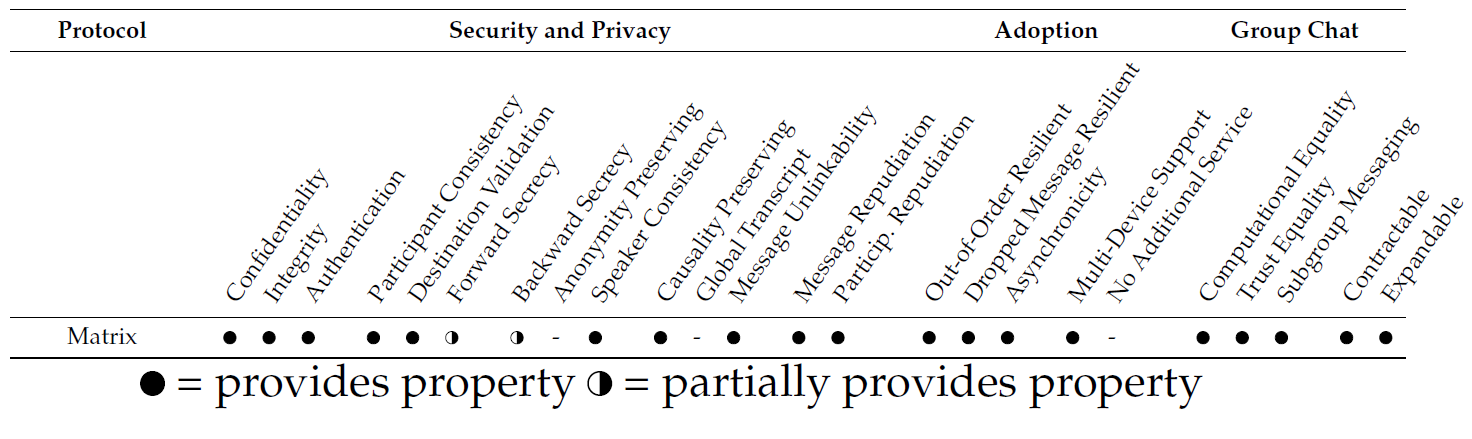
\includegraphics[width=12cm]{figures/framework.png}
	\caption{Evaluation of Matrix Security.}
	\label{fig:framework}
\end{figure}

\subparagraph{Confidentiality} When a message is sent using the Signal Protocol then only the intended recipient can read the message. The senders sending ratchet and receivers receiving ratchet will derive the same message key hence only the two parties will be able to encrypt the messages. 

\subparagraph{Integrity} The receiver will only accept a message if it is successfully decrypted hence if in transit a message was modified then the message would be rejected.

\subparagraph{Authentication} The decryption of a message also gives authentication guarantees since only the intended recipient could compute the message key.

\subparagraph{Forward secrecy} The symmetric ratchet ensures forward secrecy. If a chain session key is compromised then the previous keys can not be generated since the ratchet is one way cryptographic hash function hence secrecy is provided for all previous send messages.  

\subparagraph{Backward secrecy} Diffie-Hellman ratchet have the self-healing property and will generate a new chain session key for the symmetric ratchet hence if a chain key is compromised then secrecy for future messages is still provided because a new chain ratchet key will be generated.

\subparagraph{Anonymity preserving}

Anonymity preservation is lost in the Signal Protocol since the initial key agreement requires long-term public keys hence making them observable during Triple-DH. However \textbf{\emph{participant consistency}} is provided by Triple-DH \cite{sok}. %How?
%Without participant consistency, identity misbinding attacks might be possible. Unknown key share attack

\subparagraph{Speaker consistency}
This property is partially provided through the key evolution of the ratchets. If a message is dropped then it is not possible to generate message keys for future messages. This also makes the protocol partially have the property \emph{\textbf{Dropped message resilence}}. It will also not go unnoticed if a message is received out of order since this will result in the message's key being an unexpected key. Hence the recipient have to store expired keys to decrypt delayed messages. This makes the property \emph{\textbf{Out-of-order resilient}} only partially provided \cite{sok}.

\subparagraph{Global transcript} 
In an asynchrounous messaging protocol there is no global transcript. Both participants have to be online to receive messages hence the participants will not have all the messages if one of them is offline. This is a result of having the \textbf{\emph{Asynchronicity}} property.

\subparagraph{Deniability properties}

Since the ratchet session keys are used for encrypting messages and not the long-term public keys the properties \textbf{\emph{Message unlinkability}} and \textbf{\emph{Message repudiation}} are provided. 


\subparagraph{Other properties}

\begin{itemize}
	\item \textbf{\emph{Participant repudiation}}. Triple-DH achieves full participant repudiation since anyone can forge a transcript between any two participants \cite{sok}.
	\item \textbf{\emph{Destination validation}}. The Deffie-Hellman ratchet provides this property since the recipients public key is used to generate the chain key \cite{sok}. % Is this true?
\end{itemize}


\paragraph{Security flaw or feature?}


\subsection{End-to-end security}
It can be argued that some of the Matrix shortcomings can be configured on the application layer. This puts a lot of responsibility on the application and that it is configured correctly. 

Even if the application using Matrix is configured correctly and give the best guarantee of forward and backward secrecy this not the end of security. 

Dynamic policies?


\begin{figure}[H]
	\centering
	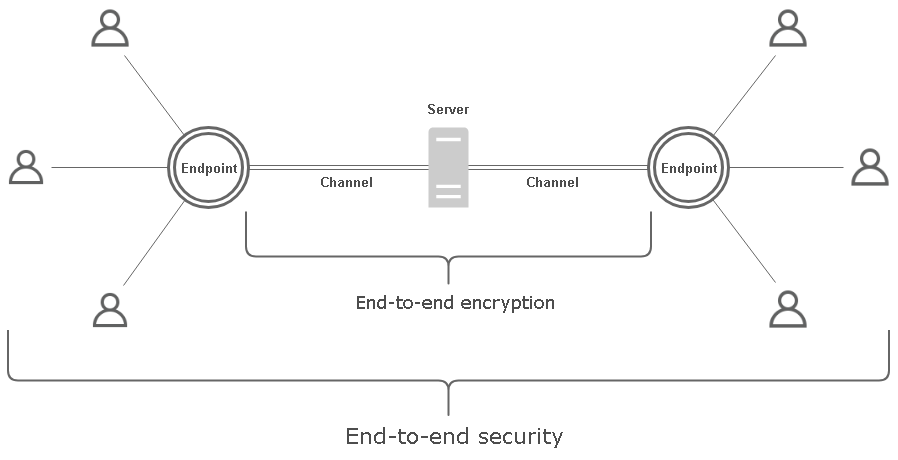
\includegraphics[width=12cm]{figures/e2esecurity.png}
	\caption{End-to-end security.}
	\label{fig:e2esecurity}
\end{figure}


Recently two technical directors from the Government Communication Headquarters of United Kingdom released an essay arguing that the software vendors could grant access to group chat by inserting the government as a hidden silent participant in a chat hence not weakening the encryption \cite{gchq}.


Explain how some of the shortcomings in Matrix can be solved with IFC.The initial state ratchet is never ratcheted?

\subsection{Summary}






% Tools issue: java sdk for matrix is beta and not fully implemented. 
% Best supported sdk is for javascript or python. Problem of running javascript code or python code with Paragon (java)
% Maybe better to use JSFlow instead 


%\section{Survey of IFC Tools}
%Having established that end-to-end security is not the end of security we will now look at Information-Flow Control tools. 

%The approach to the section will be from a programmers perspective hence usability and practicality will play a role in which IFC tool is chosen. 

%\subsection{JIF}

%\subsection{Paragon}

%\subsection{JSFlow}
%Not possible to use Matrix library with JSFlow because of missing support for libaries such as require (in node). Also overhead with configuring JSFlow to be the interpretor.

%Swift, SIF, FlowR, JFlow, LIO


%\subsection{Selection of IFC tool}
%The selection of the IFC tool used for developing the prototype is based the following defined parameters.
%The selection of IFC tool put emphasis on the practical usage in combination with Matrix. 

%\subsection{Paragon analysis}

%\subsection{Summary}


%\section{Summary}
%In this chapter the Matrix security model has been evaluated. Matrix provides end-to-end security and uses the Double Ratchet algorithm by Signal. The evaluation found that there are no major flaws in the design. To achieve end-to-end security the endpoints need to be secured as well \cite{Sabelfeld2003} this leads us to the chapter's second part. The chapter analyzed information-flow control tools and justifies the selection of Paragon which the prototype is programmed in. 